\documentclass[en,hazy,blue,screen,14pt]{elegantnote}
\usepackage[T1]{fontenc}
\usepackage[latin9]{inputenc}
% \usepackage[USenglish]{babel}
\usepackage{babel}
\usepackage{float}
\usepackage{textcomp}
\usepackage{amsmath,amsfonts,amssymb}
\usepackage{amsthm}
\usepackage{graphicx}
\usepackage[ruled,vlined]{algorithm2e}
\PassOptionsToPackage{normalem}{ulem}
\usepackage{ulem}
\usepackage{mathtools}
\usepackage{url}
\usepackage{hyperref}
\renewcommand\qedsymbol{$\blacksquare$}

\DeclarePairedDelimiter{\ceil}{\lceil}{\rceil}
\newcommand\tab[1][1cm]{\hspace*{#1}}
\newenvironment{claim}[1]{\par\noindent\underline{Claim:}\space#1}{}
\newenvironment{claimproof}[1]{\par\noindent\underline{Proof:}\space#1}{\hfill $\blacksquare$}

\title{Class Notes: STAT 501\\ Nonparametrics \& Log-Linear Models \\Hypothesis Testing}
\author{Da Kuang}
\institute{University of Pennsylvania}
% \version{1.00}
\date{}

\begin{document}

\maketitle
\newpage
\section{Big Picture}
The statistical analysis is consist of three key components.
\begin{itemize}
	\item Descriptive analysis
		\begin{itemize}
			\item mean, median, variance, standard deviation, quantile, IQR
			\item tables
			\item graphs
		\end{itemize}
	\item Statistical inference
		\begin{itemize}
			\item Point estimation
			\item Hypothesis testing
			\item Confidence interval
		\end{itemize}
	\item Model diagnostics.
\end{itemize}

In this lecture, we will focus on reviewing Hypothesis Testing.
\section{Hypothesis Testing}
\section{Parametric Method}
We associate parametric distributions with populations. For instance, $N(\mu, \sigma^2)$, $\text{binomial}(n, p)$. So we make inference about the unknown parameters.

For example,
\begin{itemize}
	\item $X_i, i = 1, \dots, n$, iid from $N(\mu, \sigma^2)$.
	\item $\hat{\mu} = \bar{X} = \frac{1}{n} \sum_{i=1}^{n}X_i$.
	\item $\hat{\sigma}^2 = \frac{1}{n-1} \sum_{i=1}^{n}(X_i - \bar{X})^2$.
\end{itemize}

\subsection{Population variance and sample variance}
Why we have $n-1$ in the denominator for sample variance?
Answers:
\begin{itemize}
	\item Concise but not helpful answer: Bessel's correction.
	\item Intuitive but over-simplified answer: overcome underestimation.
	
	We are trying to use the sample variance to estimate the population variance. The estimator of variance is consistent but biased because it is based on the estimator of mean. The freedom of the variance is actually not $n$ but $n-1$. So we can overcome the underestimation by dividing by $n-1$.
	\item To have a more thorough explanation, check \href{https://en.wikipedia.org/wiki/Variance#Population_variance_and_sample_variance}{the Wikipedia of Variance}.
\end{itemize}

\subsection{\texttt{pnorm} and \texttt{qnorm}}
\begin{itemize}
	\item \texttt{pnorm(-1.645) \# 0.04998491}
	\item \texttt{qnorm(0.05) \# -1.645}
	\item lower.tail: logical; if TRUE (default), probabilities are $P[X \le x]$ otherwise,
$P[X > x]$.
\end{itemize}

In the following figure, on the left is the lower quantile and on the right is the upper quantile.

\begin{figure}[H]
	\centering
	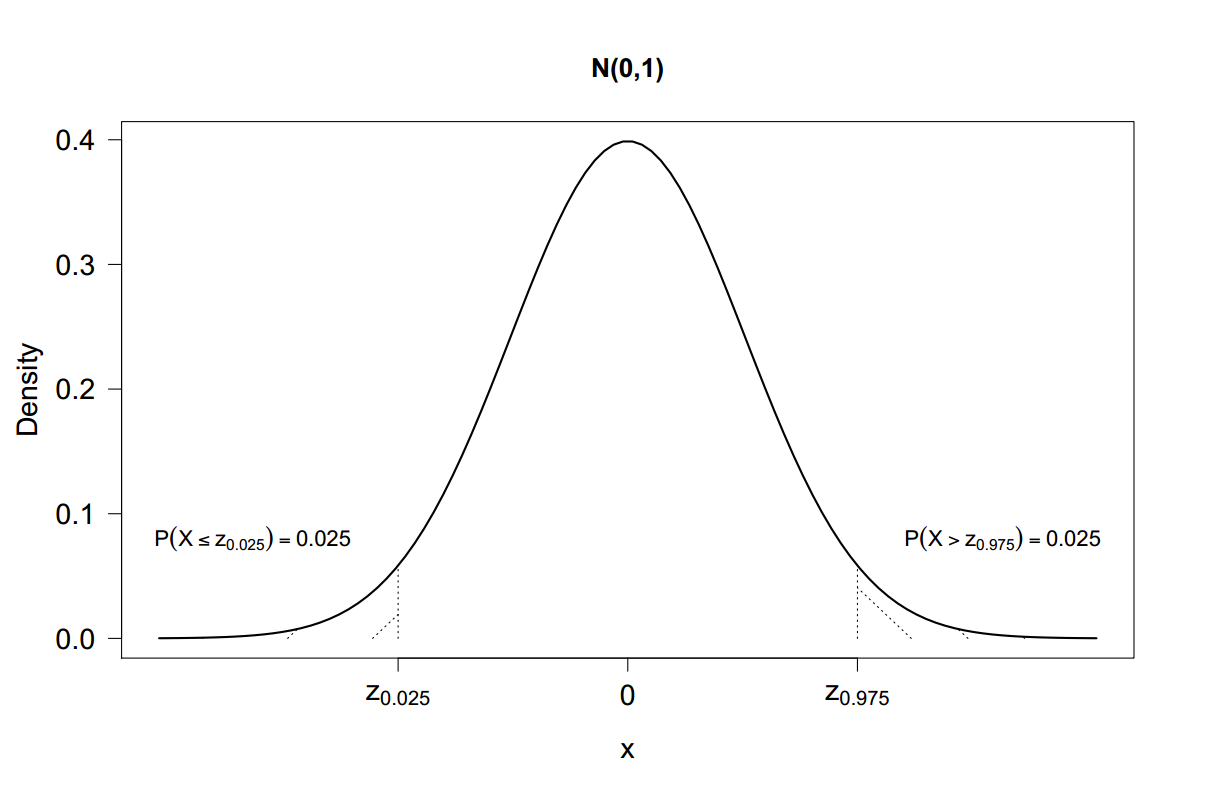
\includegraphics[width=0.5\linewidth]{fig/norm-distribution}
	\caption{}
	\label{fig:norm-distribution}
\end{figure}
\subsection{student's t-distribution}
\subsection{One-sided $H_1$}
\subsection{Two-sided $H_1$}
\end{document}
